% Chapter 3: Proposed System

\chapter{Proposed System} \label{chap3}
\newpage

This chapter states the problem that motivated the project, defines what the work does and does not cover, and describes the proposed system: its architecture, agents, document pipeline, event flow, use cases and technology choices.

\section{Problem Statement}
In most organisations the IT procurement process is a chain of loosely connected manual steps. A purchase order or invoice arrives in whatever form the vendor chose, someone retypes its contents into a system, someone else checks the vendor, and an approval request travels by e-mail until somebody replies. Contracts are filed with their renewal dates noted on a calendar, and software licences are renewed without checking whether anyone still uses them. Each step is slow on its own, and together they leave room for costly mistakes and for fraud. Table~\ref{tab:problems} lists the main problems and their impact.

\begin{table}[!htbp]
\centering\tablestyle
\caption{Problems in the current procurement process and their impact}\label{tab:problems}
\begin{tabularx}{\textwidth}{|L{0.46\textwidth}|Y|}
\hline
\textbf{Problem} & \textbf{Impact} \\ \hline
Documents arrive through disconnected channels in inconsistent formats & Manual data entry, delays and extraction errors \\ \hline
Vendor records are not de-duplicated and payment-detail changes are accepted on request & Duplicate vendors, BEC fraud and payments to the wrong account \\ \hline
Approvals are routed by hand with no SLA or stock checks & Stalled requests, overspending and two requests consuming the same stock \\ \hline
Software licence usage is not monitored, or is judged by a flat inactivity rule & Money spent on unused seats, or seats reclaimed by mistake \\ \hline
Contract terms are tracked informally & Silent auto-renewals and missed notice periods \\ \hline
Vendor risk is assessed once, at onboarding & Stale risk ratings \\ \hline
No single view of a request across tools & Difficult auditing and slow investigation of problems \\ \hline
\end{tabularx}
\end{table}

These problems are connected. A vendor record that was never checked is exactly what makes a fraudulent bank-detail change possible, and an extraction error that goes unnoticed can become a duplicate payment, so fixing one step in isolation helps only a little. The problem addressed in this project is therefore: \textit{to design and build an automated, event-driven procurement platform that reads unstructured procurement documents, links every document to a vendor record, routes approvals under spend and deadline controls, manages contracts and renewals, and keeps a vendor risk score up to date, while keeping automated decisions explainable and auditable and keeping a person in the loop for low-confidence results and sensitive changes.}

\section{Scope}\label{sec:scope3}
The project covers the path from an incoming procurement document or purchase request to a signed contract, the receipt of goods and the matching of the vendor's invoice. Within this scope the system scans and reads documents, matches vendors, routes approvals with spend-tier and SLA controls, checks each request against its department's budget, reserves inventory, monitors licence usage, offers an IT catalog with agreed prices, runs request-for-quotation events, records partial deliveries, checks invoices for GST and computes TDS, generates, signs and tracks contracts and the obligations they contain, scores vendor risk and keeps a performance scorecard per vendor, and keeps users informed through e-mail notifications, all behind role-based access control and with metrics, logs and an audit trail.

The work does not include payment execution, ERP integration, live GSTIN registry and news lookups as a default (the clients exist but are switched off, so adverse-media screening reads a sample feed in the demonstration), a third-party e-signature provider in the demonstrated configuration (Documenso and DocuSign clients exist but signing is done in the application), automatic retraining of models, or a production or Kubernetes deployment. All data is synthetic: the vendor risk training set, the licence usage logs, the classifier corpus and the sample documents are generated, and the CUAD contracts are used only to evaluate clause extraction.

\section{Scope Design}
The system design defines the structure, components, interfaces and information flow of the platform. Its scope covers the following areas:
\begin{itemize}
  \item \textbf{System architecture:} the user interface, gateway, agent services, event bus, data stores and their relationships.
  \item \textbf{User interface design:} role-specific pages through which users submit requests, review extracted data, approve or reject requests, sign contracts and inspect vendors, licences and notifications.
  \item \textbf{Agent coordination:} how the agents cooperate through events, for example from document intake to purchase request, approval, contract and notification.
  \item \textbf{Data flow:} how information moves from user input through processing and analysis to stored records and messages.
  \item \textbf{External dependencies:} ClamAV signature updates, an SMTP service (Mailpit in development), the HaveIBeenPwned password range API, a public IFSC directory, the Frankfurter exchange-rate API, the OpenSanctions consolidated list, Hugging Face model downloads, and a local Ollama model for the assistant.
  \item \textbf{Output and decision support:} confidence scores, risk bands with contributing factors, anomaly reasons for licences, and the risk shown to a signer before signing.
\end{itemize}
The system assists procurement decisions and does not guarantee correct extraction, which is why low-confidence results are sent to human review.

\section{Proposed System}

\subsection{Overview and Architecture}
The proposed system is an event-driven platform of four cooperating agents. Each agent is one or more independent FastAPI services with their own data and responsibilities, and the agents communicate mainly through events on a Kafka-compatible bus (Redpanda) rather than by calling one another. Users reach the system through a React frontend and an Nginx gateway; every service verifies the caller's JWT and role itself. The services share one PostgreSQL database, in which each service owns and migrates its own tables, together with Redis for locks and caching and MinIO for document files. Figure~\ref{fig:arch} shows the overall structure.

\begin{figure}[!htbp]
\centering
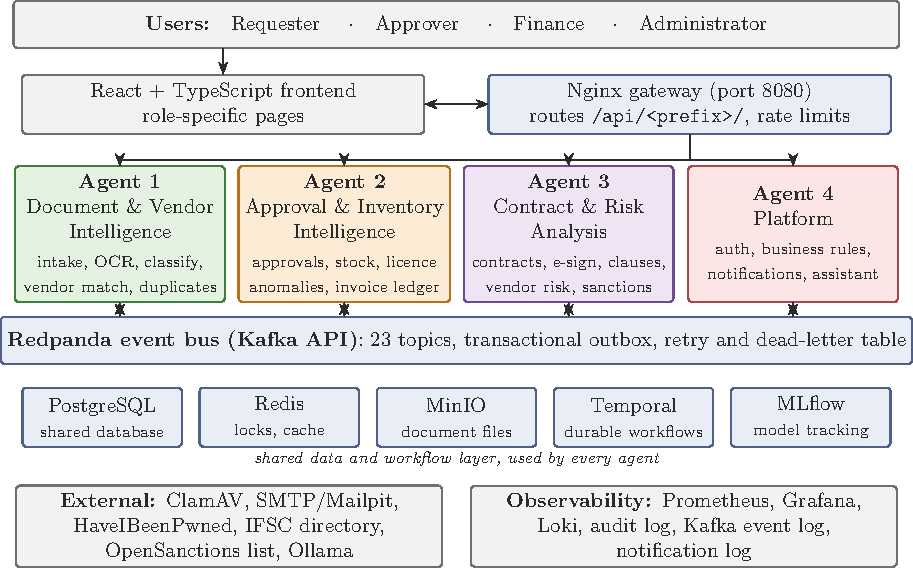
\includegraphics{figures/diagrams/arch}
\caption{Overall architecture of the proposed system}\label{fig:arch}
\end{figure}

This decomposition isolates concerns: a change to extraction does not touch the approval engine, and a slow parse cannot block an upload, because heavy work runs in background workers off the request path.

\subsection{The Four Agents}
Table~\ref{tab:agents} summarises the agents, and the paragraphs that follow describe what each one does. In the sense defined in Section~\ref{sec:agentdef}, each agent observes events, decides within the limits set by the business rules, acts, and defers to a person when its confidence is low or the action is sensitive.

\begin{table}[!htbp]
\centering\tablestyle
\caption{Summary of the four agents in the proposed system}\label{tab:agents}
\begin{tabularx}{\textwidth}{|L{0.17\textwidth}|L{0.11\textwidth}|L{0.30\textwidth}|Y|}
\hline
\textbf{Agent} & \textbf{Port} & \textbf{Main responsibility} & \textbf{Key techniques} \\ \hline
Document and Vendor Intelligence & 8001 (+ worker) & Document intake, reading, classification, field extraction, vendor matching and onboarding, duplicate detection, bank-detail control & ClamAV, pdfplumber, Docling, PaddleOCR, TF-IDF + logistic regression, LayoutLMv3, rapidfuzz \\ \hline
Approval and Inventory Intelligence & 8002 (+ worker) & Approval routing and authority, SLA escalation, inventory reservation and reorder, licence anomalies and reclaim, invoice ledger & Temporal, Redis locks, Isolation Forest, SHAP \\ \hline
Contract and Risk Analysis & 8003 (+ worker) & Contract generation and signing, clause extraction, renewal reminders, vendor risk scorecard and clearance, sanctions screening, offboarding & Jinja2, Legal-BERT (CUAD), deterministic ruleset engine \\ \hline
Platform & 8004, 8005, chatbot & Authentication and roles, business-rules engine, notifications, conversational assistant & JWT, argon2id, Jinja2, SMTP, Ollama (Llama 3.2 3B) \\ \hline
\end{tabularx}
\end{table}

\paragraph{Document and Vendor Intelligence.} This agent is the entry point for every document, whether uploaded, e-mailed to an intake address or dropped into a watched folder. It checks the file's size and real type, streams it through ClamAV and rejects it if the scanner flags it or cannot be reached, stores it in MinIO and publishes \code{document.ingested} in the same database transaction. A background worker reads, classifies and extracts the document, gives every field a confidence score and sends doubtful results to a review queue. Each invoice is also checked for GST: the supplier's GSTIN, the split between central, state and integrated tax, the rate expected for each HSN or SAC code, the totals and, where present, the signed e-invoice QR code; a failed check forces review but never changes the confidence score. The agent matches the vendor against existing records, books invoices against their purchase request, flags likely duplicates, and never applies new bank details directly: they wait as a pending change until a different user with the finance or admin role verifies them, and payment is held meanwhile.

\paragraph{Approval and Inventory Intelligence.} This agent derives each request's approval chain from spend tiers held in the business-rules engine (automatic up to \Rs 500, a department manager up to \Rs 5,000, and a manager plus the finance head above that) and from an approval-authority matrix that also enforces separation of duties: nobody, including an administrator, can approve their own request. A Temporal workflow per request waits for the decision, reminds the approver at 50\% and 80\% of the SLA and escalates after 48 hours. Stock is reserved under a short Redis lock so that two concurrent requests cannot take the last unit, and a request for an item that is out of stock is created as back-ordered. An Isolation Forest scores licence usage; a licence above the anomaly threshold receives a reclaim request that waits through a seven-day grace period before it reaches an approver. When \code{contract.signed} arrives, the request moves to \emph{ordered}; deliveries are then recorded per line, with asset tags for hardware (\emph{partially received} until everything has arrived, then \emph{fulfilled}), and invoices are matched line by line against the order, with a 1\% tolerance on the unit price and on the order's remaining balance before an invoice is held; once deliveries are recorded, an invoice may not exceed the quantity received. When an invoice is booked, the TDS to deduct is computed from the vendor's or the category's section and threshold. Each new request is also checked against its department's budget for the category and fiscal quarter, and the agent maintains the IT catalog and request-for-quotation events (Section~\ref{sec:extensions}).

\paragraph{Contract and Risk Analysis.} When a request is approved, this agent fills one of three Jinja2 templates (hardware purchase, SaaS subscription or professional services), renders the contract as text and PDF, and sends it for signature automatically. Signing happens in the application: an authorised approver, finance or admin user types or draws a signature, gives consent, and the contract and signer details are sealed with a SHA-256 hash recorded in the audit log and shown on a signature certificate. If the vendor is rated High or has not been scored, the signer must explicitly acknowledge the risk. An HMAC-verified, replay-protected webhook accepts signatures from external providers and is used by the tests. A Legal-BERT model reads the renewal term, notice period and expiration date from the contract text, and a Temporal workflow sends renewal reminders 60, 30 and 15 days before the notice deadline. After signature it reads the obligations the contract contains (Section~\ref{sec:extensions}). The agent also scores each vendor's risk with a deterministic 100-point scorecard, answers whether a vendor is cleared for activation, a purchase or a contract (taking human decisions such as an accepted risk into account), keeps a performance scorecard per vendor, screens vendor names against a sanctions list and news results for adverse media, and handles vendor offboarding by flagging active contracts for review instead of closing them. Every risk score stores its inputs and a SHA-256 hash, so it can be replayed exactly; evidence and disputes from vendors or staff are kept with the score.

\paragraph{Platform.} The fourth agent owns what no functional agent should. The authentication service issues 15-minute JWT access tokens and refresh tokens held in an httpOnly cookie (revoked on logout), hashes passwords with argon2id, verifies e-mail addresses, locks an account after repeated failures and rejects passwords found in known breaches. It also hosts the business-rules engine: 71 rules, such as spend tiers, thresholds and tolerances, that an administrator edits at run time and that services refresh when \code{business_rule.updated} is published. The notification service consumes 17 event topics, sends urgent messages immediately and batches routine ones into digests, retries failed deliveries and logs every message. Finally, a conversational assistant answers questions by retrieval-augmented generation with a local Llama~3.2 (3B) model through Ollama. An index of contract clauses, document text, business rules and current records (requests, vendors, licences, budgets) is embedded with \code{nomic-embed-text} into PostgreSQL with pgvector and kept current every minute; for each question the closest passages the user is allowed to see are retrieved and the model answers only from them, citing their source, and says so when they do not contain the answer. Access is applied when retrieving (staff see everything; a requester only their own requests, contracts and documents), and bank details are masked before indexing.

\subsection{Extensions after the Competitive Analysis}\label{sec:extensions}
The comparison with commercial suites (Section~\ref{sec:commercial}) identified capabilities that matter for IT procurement and that the platform lacked. Five were added without changing the existing flow: each is switched off or advisory by default, uses the existing agents, events and business rules, and is described in Table~\ref{tab:extensions}.

{\tablestyle
\begin{longtable}{|L{0.17\textwidth}|L{0.47\textwidth}|L{0.26\textwidth}|}
\caption{Extensions added after the competitive analysis}\label{tab:extensions}\\
\hline
\textbf{Extension} & \textbf{Behaviour} & \textbf{Agent and rules} \\ \hline
\endfirsthead
\multicolumn{3}{l}{\small\textit{Table \thetable\ (continued)}}\\ \hline
\textbf{Extension} & \textbf{Behaviour} & \textbf{Agent and rules} \\ \hline
\endhead
Budget control & A budget is set per department, IT category (hardware, software, SaaS, services) and fiscal quarter. Its usage is computed from the requests that refer to it---pending, committed after approval, consumed once invoiced---so rejections and cancellations release money without bookkeeping. The budget row is locked while a request is checked, so two concurrent requests cannot both use the last amount. A request that would exceed the budget gets a finance approval step. & Approval and Inventory; seven \code{budget.*} rules \\ \hline
Contract obligations & After signature the contract is read for eleven obligation types: SLA uptime and service credits, licence limits, price-increase cap, audit rights, warranty, termination for convenience, minimum commitment, exit terms, data protection, liability cap and insurance. Each finding waits for a person to confirm it; confirmed obligations get a due date and reminders. Recording a month's measured uptime computes the service credit, and invoices for the request carry a note until the credit is applied. A licence with more users than the contract allows is marked as breached, and licence reclaims respect a minimum commitment. & Contract and Risk;\newline \code{contract.obligation_*},\newline \code{contract.sla_credit_}\newline\code{auto_expect} \\ \hline
IT catalog & Approved items with an agreed price, vendor, lead time, warranty and expiry date. A catalog line takes its price, vendor and request type from the catalog, not from the client; an expired item cannot be ordered. A seat add-on increases the licence's seat count when it is received. Catalog-only requests up to a set amount can skip the manager step. & Approval and Inventory;\newline \code{catalog.preapproved_}\newline\code{max_inr} \\ \hline
Sourcing events (RFQ) & A buyer invites two or more vendors to quote by a deadline. A quote that carries the RFQ reference is linked automatically when the document pipeline reads it. While an RFQ is sealed, no role sees amounts before the deadline. Quotes are scored per criterion---price, lead time, warranty, support, vendor risk band and on-time delivery---and weighted; a shortlist can go to a second round, and the award creates the purchase request. Requests above a threshold without an RFQ or catalog price are flagged. & Approval and Inventory; \code{sourcing.*} \\ \hline
Partial receipts and scorecards & Deliveries are recorded per line with asset tags; an invoice for more than has been received is a variance, completing the three-way match. A scorecard per vendor reports on-time delivery, invoice accuracy, RFQ response rate and SLA breaches, and feeds the RFQ comparison. & Approval and Inventory\newline (\code{invoice.match_}\newline\code{against_received});\newline Contract and Risk \\ \hline
GST and TDS & Every invoice is checked for GST: supplier GSTIN, central and state tax or integrated tax depending on the place of supply, the rate for each HSN or SAC code, and taxable value plus tax equal to the total; reverse charge applies to services from suppliers outside India. An e-invoice QR code is verified against the tax portal's public key and compared with the printed invoice. A failed check forces review and publishes \code{invoice.tax_flagged}, without changing the confidence score. TDS is computed when an invoice is booked, the GSTR-2B statement from the GST portal is reconciled with the books, and payment deadlines for micro and small enterprises are tracked. The rates are seeded values that a chartered accountant must confirm. & Document and Vendor; Approval and Inventory;\newline \code{gst.*}, \code{tds.*}, \code{msme.*} \\ \hline
\end{longtable}}

\subsection{Document Processing Pipeline}
The document pipeline turns an uploaded file into a structured, confidence-scored record (Figure~\ref{fig:pipeline}). The upload returns as soon as the file is stored; a worker processes it in the background.

\begin{figure}[!htbp]
\centering
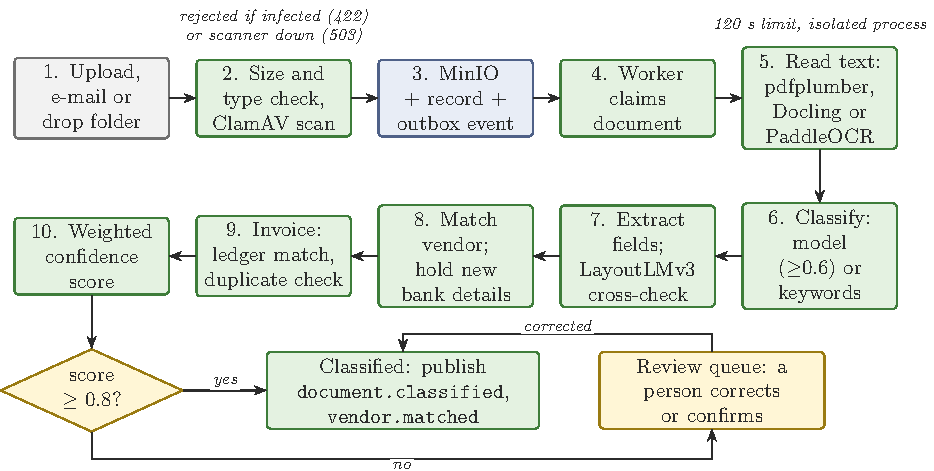
\includegraphics{figures/diagrams/pipeline}
\caption{Document processing pipeline of the Document and Vendor Intelligence agent}\label{fig:pipeline}
\end{figure}

A file is rejected before storage if it is empty, too large (25\,MB at the gateway), of a type that its bytes do not confirm, infected, or if ClamAV cannot be reached, so the intake fails closed. After the file and its database row are stored, the worker reads it in a separate process with a 120-second limit: pdfplumber for PDFs with a usable text layer, Docling for scanned PDFs, and PaddleOCR for images after deskewing and upscaling by at most 1.5 times. The classifier labels the document as an invoice, purchase order, quotation or other paperwork, and regular expressions extract the vendor name, document number, date, currency, totals and line items. When LayoutLMv3 is installed it reads the document independently, and a disagreement forces review. The vendor name is normalised and matched against existing vendors with a fuzzy ratio of at least 88, or a new vendor record is created; first-seen bank details are held for verification. An invoice is booked against its purchase request and checked for duplicates: same vendor, an amount within 2\%, a date within 7 days and a document number at least 85\% similar (all three values are business rules). Finally, the per-field confidence scores are combined into an overall score (Section~\ref{sec:code}); a document scoring below 0.8 goes to the review queue, and reviewers' corrections are kept as per-vendor hints for later documents. Any dependency failure returns the document to the queue to be retried, up to five attempts.

\subsection{Inter-Agent Communication and Workflow}
Every event uses the same envelope (event ID, event type, timestamp, source service, correlation ID and payload), and the 23 topics and their payloads are fixed in a shared contract document so that producers and consumers could be built in parallel. Each service authenticates to the broker with its own SASL/SCRAM account and may use only its own topics. Events are written to an outbox table in the same transaction as the change that caused them and relayed to the broker afterwards; consumers are idempotent, retry failures and move events that keep failing to a dead-letter table shown on the Control Panel. Figure~\ref{fig:events} shows the main flows and Table~\ref{tab:events} lists the topics.

\begin{figure}[!htbp]
\centering
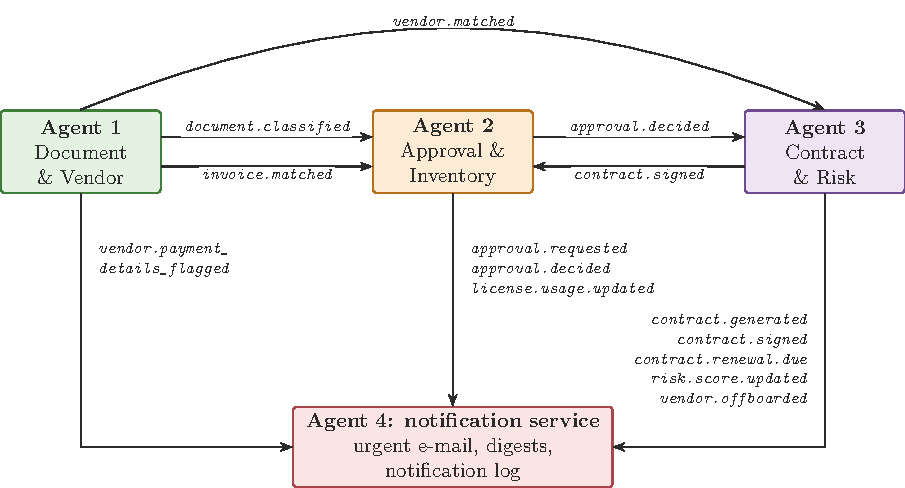
\includegraphics{figures/diagrams/events}
\caption[Main event flows between the agents]{Main event flows between the agents. Rule changes (\code{business_rule.updated}) are broadcast to every agent and are omitted for clarity.}\label{fig:events}
\end{figure}

\begin{longtable}{|L{0.36\textwidth}|L{0.13\textwidth}|L{0.41\textwidth}|}
\caption{Event topics exchanged between the agents}\label{tab:events}\\
\hline
\textbf{Topic} & \textbf{Published by} & \textbf{Consumed by and purpose} \\ \hline
\endfirsthead
\multicolumn{3}{l}{\small\textit{Table \thetable\ (continued)}}\\ \hline
\textbf{Topic} & \textbf{Published by} & \textbf{Consumed by and purpose} \\ \hline
\endhead
\code{document.ingested} & Agent 1 & Agent 1 worker: starts the pipeline \\ \hline
\code{document.classified} & Agent 1 & Agent 2: turns a quote into a purchase request; notifications \\ \hline
\code{vendor.matched} & Agent 1 & Agent 3: scores the vendor's risk \\ \hline
\code{vendor.payment_}\newline\code{details_flagged} & Agent 1 & Notifications: urgent alert on a pending bank-detail change \\ \hline
\code{invoice.matched} & Agent 1 & Agent 2: updates the invoice ledger and request status \\ \hline
\code{approval.requested} & Agent 2 & Notifications: tells the approver \\ \hline
\code{approval.decided} & Agent 2 & Agent 3: generates the contract; Agent 1: books invoices waiting for the request; notifications \\ \hline
\code{license.usage.updated} & Agent 2 & Notifications: utilisation and anomaly alerts \\ \hline
\code{order.summary.generated} & Agent 2 & Control Panel: hourly open-order summary \\ \hline
\code{contract.generated} & Agent 3 & Notifications \\ \hline
\code{contract.signed} & Agent 3 & Agent 2: request becomes \emph{ordered}; notifications \\ \hline
\code{contract.renewal.due} & Agent 3 & Notifications: 60, 30 and 15-day reminders (urgent at 15) \\ \hline
\code{risk.score.updated} & Agent 3 & Notifications: urgent for the High band \\ \hline
\code{vendor.offboarded} & Agent 3 & Notifications: offboarding summary and contracts flagged \\ \hline
\code{reminder.due} & Agents 1--3 & Notifications: reminder to whoever must act; Control Panel \\ \hline
\code{business_rule.updated} & Agent 4 & Agents 1--3: refresh their cached rules \\ \hline
\code{notification.send} & Any service & Notifications: generic message \\ \hline
\code{budget.threshold_crossed} & Agent 2 & Notifications: budget warning or overrun \\ \hline
\code{rfq.issued} & Agent 2 & Notifications: invitation to each invited vendor \\ \hline
\code{rfq.awarded} & Agent 2 & Notifications: award and thank-you messages \\ \hline
\code{goods.received} & Agent 2 & Notifications: delivery recorded \\ \hline
\code{contract.obligation.due} & Agent 3 & Notifications: obligation due, overdue or breached \\ \hline
\code{invoice.tax_flagged} & Agent 1 & Control Panel: failed GST check \\ \hline
\end{longtable}

In a typical run, a requester creates a purchase request, or a vendor quote is dropped into the intake folder and Agent~1 classifies it and Agent~2 creates the request from it. Agent~2 builds the approval chain and, once the last approver agrees, publishes \code{approval.decided}. Agent~3 generates the contract and sends it for signature, and its \code{contract.signed} event moves the request to \emph{ordered}. The notification service follows all of these events, sending urgent alerts such as an approval request or a flagged bank-detail change immediately and batching routine ones into a digest. Every API request receives a correlation ID at the gateway, which is carried through the events and log lines of every service, so the whole journey of one request can be followed in Grafana.

\subsection{Use Case View}
Figure~\ref{fig:usecase} presents the use cases of the four roles. The \emph{Requester} raises purchase requests, uploads documents and follows their progress; the \emph{Approver} decides the requests and licence reclaims assigned to them in the approval-authority matrix and can sign contracts; the \emph{Finance} user verifies bank-detail changes, onboards vendors, maintains risk signals and can also approve and sign; and the \emph{Administrator} manages users and business rules, monitors the system and offboards vendors. Administrators can perform every action, so the diagram shows each role only with the actions specific to it.

\begin{figure}[!htbp]
\centering
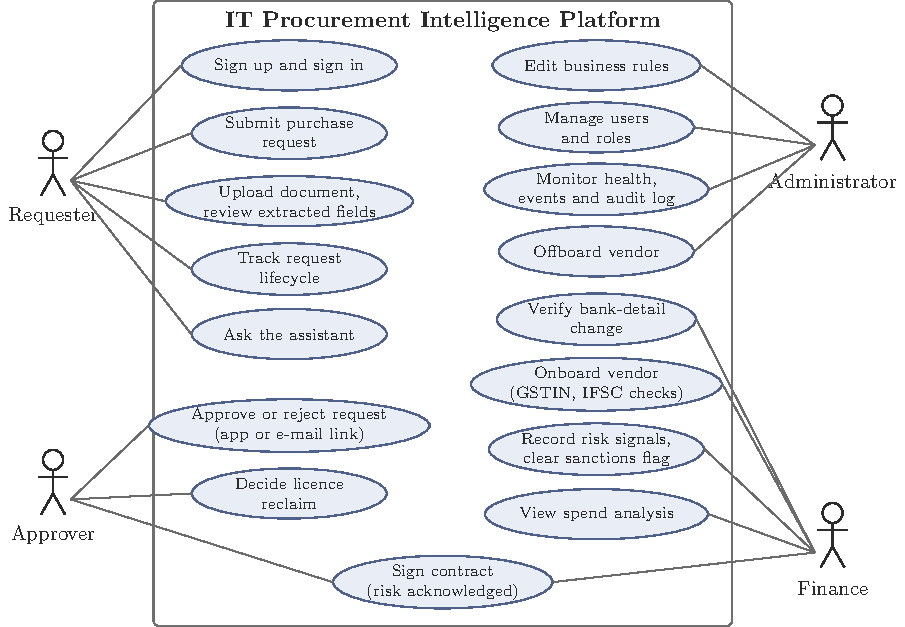
\includegraphics{figures/diagrams/usecase}
\caption{Use case diagram of the IT procurement platform}\label{fig:usecase}
\end{figure}

The use cases group into five phases:
\begin{enumerate}
  \item \textbf{Authentication and business rules.} Users sign up, verify their e-mail and sign in; an administrator assigns roles and edits the business rules (spend tiers, SLA, thresholds and tolerances) on the Business Rules page, with every change kept in a history.
  \item \textbf{Purchase and inventory.} A requester submits a purchase request, stock is checked and reserved, the approval workflow runs in Temporal, and the approver approves or rejects.
  \item \textbf{Vendor intelligence.} Vendor documents are read and matched, new vendors are onboarded with identifier checks, bank details are verified by a second person, and a vendor risk score is calculated.
  \item \textbf{Contract and risk.} A contract is generated for the approved request, sent for signature, signed in the application after the vendor's risk is shown, and renewal reminders are scheduled.
  \item \textbf{Notification.} Approvals, flagged bank details, renewals, risk changes and signatures trigger e-mail notifications to the people concerned.
\end{enumerate}

\subsection{Key Design Principles}
Four principles run through the design. The system is \emph{fraud-aware}: uploads are scanned and rejected if the scanner is unavailable, bank details need a second person's verification, the webhook is accepted only with a valid HMAC signature and never twice, and signing a contract with a High-risk vendor requires an explicit acknowledgement. It is \emph{human-centred}: results below the confidence threshold go to review, a licence reclaim waits for the holder and an approver, offboarding flags contracts rather than closing them, and the models never retrain themselves. It is \emph{accountable}: significant actions are written to an audit log, identity is always taken from the JWT and never from a request body, business-rule changes are versioned, and every model-routing decision is logged. Finally, it is \emph{observable}: every service exposes Prometheus metrics, logs carry a correlation ID, the Control Panel shows every Kafka event and every failed event, and a System Health page shows the state of the services.

\subsection{Technology Stack}
Table~\ref{tab:stack} lists the main technologies. Pretrained open-source components are used wherever possible; the models trained within the project are the document classifier, the licence-anomaly model and the vendor risk model.

\begin{table}[!htbp]
\centering\tablestyle
\caption{Technology stack of the proposed system}\label{tab:stack}
\begin{tabularx}{\textwidth}{|L{0.18\textwidth}|L{0.38\textwidth}|Y|}
\hline
\textbf{Layer} & \textbf{Technology} & \textbf{Purpose} \\ \hline
Frontend & React, TypeScript, Vite, Tailwind CSS & Role-based pages, one home page per item \\ \hline
Gateway & Nginx & Single entry point; routes \texttt{/api/<prefix>/}, rate limits, security headers \\ \hline
Backend services & FastAPI (Python), SQLAlchemy, Alembic, Docker Compose & One containerised service per agent, plus workers \\ \hline
Messaging & Redpanda (Kafka API), aiokafka, SASL/SCRAM & Events between agents, per-service topic permissions \\ \hline
Workflow engine & Temporal & Approval SLAs, reclaim grace period, renewal reminders \\ \hline
Data stores & PostgreSQL, Redis, MinIO & Records, locks and caches, document files \\ \hline
Document AI & pdfplumber, Docling, PaddleOCR, LayoutLMv3, rapidfuzz & Text extraction, OCR, cross-check, vendor and duplicate matching \\ \hline
Models & scikit-learn (logistic regression, Isolation Forest)~\cite{pedregosa2011sklearn}, SHAP, Legal-BERT (Hugging Face Transformers), MLflow & Classification, licence anomalies, clause extraction, experiment tracking (vendor risk uses a deterministic ruleset) \\ \hline
Assistant & Ollama (Llama 3.2 3B, nomic-embed-text), PostgreSQL pgvector & Retrieval-augmented answers from contracts, documents, rules and current records, with citations \\ \hline
Security & JWT, argon2id~\cite{biryukov2016argon2}, HMAC-SHA256, ClamAV, HaveIBeenPwned & Authentication, password hashing, webhook verification, malware scanning, breached-password check \\ \hline
Monitoring & Prometheus, Grafana, Loki, Promtail, kafka-exporter & Metrics, dashboards, centralised logs by correlation ID, consumer lag \\ \hline
Notifications & Jinja2 templates, SMTP (Mailpit in development) & Templated e-mail \\ \hline
\end{tabularx}
\end{table}
